\section{Experiments \& Results}

This section describes the conducted experiments and highlights the main results, including the most promising configurations as well as their performance. It also presents the results of two small-scale ablation studies.

\subsection{Experiments Overview}

First, we needed to establish a baseline to compare methods like Mixstyle against. As mentioned previously, the two most promising backbones were ResNet-18 and ResNet-50. It is hence sensible to select their vanilla variants for this purpose. Against that baseline, we conducted three different experiments: layer freezing, Mixstyle and a combination of both. Layer freezing seemed promising as the feature extraction process in the earlier layers should be no different across the domains. Freezing those layers hence could stabilize the feature extraction for the later layers to become more domain invariant. Mixstyle does not need further introduction at this point and a combination of both could yield a more stable perturbation in the feature space. Among the configurations, the most notable parameters were which layers to freeze, after which layers to include a Mixstyle layer and what $\alpha$ to use in the Mixstyle layers.

\subsection{Effects of Configurations}

We employ freezing to enable more stable feature extraction. Freezing later layers has the consequence of reducing the model's ability to generalize to new domains. We noticed that especially freezing the last two layers decreases the performance substantially. Mixstyle is also best applied in earlier layers. Perturbing the output of later layers decreases performance, as semantic information rather than style information would be mixed in doing so.

For configurations with freezing as well as with Mixstyle, it has shown that introducing a 512-dimensional fully-connected layer right before the classification layer slightly increases performance. An explanation could be that as both methods make it harder or even impossible for earlier layers to adapt to the data, a fully-connected layer at the end balances the capacity of the model and introduces more learning capabilities in the latent space.

\subsection{Experimental Results}

\begin{table}[t]
    \centering
    \caption{Experimental results using three domains of PACS for training and one for validation. Results are given as mean $\pm$ standard deviation of the mean accuracy across three seeds. The accuracy is given in percent. The upper two models are our baseline, the models beneath are the different configurations from our experiments, all with ResNet-50 as backbone. FC means introducing a 512-dimensional fully connected layer after the feature maps. FR$x$ means freezing layer $x$. MS$x$ means introducing a Mixstyle layer after layer $x$.}
    \label{tab:results}
    \vspace{.5em}
    \adjustbox{width=\textwidth,center}{
    \begin{tabular}{l c c c c c}
        \toprule
        \textbf{Model} & \textbf{Art painting} & \textbf{Cartoon} & \textbf{Photo} & \textbf{Sketch} & \textbf{Total} \\
        \midrule
        ResNet-18 & $78.06 \pm 0.22$ & $76.51 \pm 0.51$ & $97.94 \pm 0.28$ & $66.43 \pm 1.29$ & $77.89 \pm 0.29$ \\
        \midrule
        ResNet-50 & $84.80 \pm 0.26$ & $74.53 \pm 0.22$ & $\mathbf{98.12 \pm 0.12}$ & $68.66 \pm 1.29$ & $81.53 \pm 0.41$ \\
        + FC + FR1 & $85.24 \pm 0.58$ & $71.90 \pm 1.90$ & $\mathbf{98.12 \pm 0.16}$ & $68.84 \pm 1.02$ & $81.03 \pm 0.81$ \\
        + FC + FR1\&2 & $84.13 \pm 0.38$ & $72.45 \pm 1.15$ & $97.74 \pm 0.12$ & $70.83 \pm 0.86$ & $81.29 \pm 0.15$ \\
        + FC + MS1 & $86.98 \pm 0.69$ & $75.87 \pm 0.95$ & $\mathbf{98.00 \pm 0.22}$ & $74.13 \pm 2.24$ & $83.74 \pm 0.16$ \\
        + FC + MS1\&2 & $88.77 \pm 0.63$ & $\mathbf{76.74 \pm 1.21}$ & $\mathbf{98.18 \pm 0.07}$ & $\mathbf{75.50 \pm 1.36}$ & $\mathbf{84.80 \pm 0.05}$ \\
        + FC + FR1\&2 + MS2 & $87.61 \pm 0.53$ & $74.57 \pm 2.79$ & $\mathbf{98.28 \pm 0.03}$ & $73.79 \pm 0.90$ & $83.56 \pm 0.67$ \\
        + FC + FR1 + MS1\&2 & $\mathbf{89.11 \pm 0.29}$ & $\mathbf{76.70 \pm 0.96}$ & $\mathbf{98.10 \pm 0.06}$ & $75.14 \pm 0.75$ & $\mathbf{84.76 \pm 0.49}$ \\
        \bottomrule
    \end{tabular}}
\end{table}

The results of our baseline as well as from our most promising configurations are shown in table \ref{tab:results}. First of all, note that ResNet-50 is clearly more performant than ResNet-18. That is also the reason why the rest of the experiments use ResNet-50 as their backbone. The table also shows that freezing the first two layers doesn't seem to affect the performance. Mixstyle, however, brings a substantial performance increase of about 3\%. This is also confirming the results of \cite{mixstyle_ref}. The most notable difference lies in the sketch domain, which is the hardest of the four. Here, Mixstyle even increases performance by about 7\%. The first layer is the most important one for introducing Mixstyle, as the boost in performance is most noticeable here. We had the best results with $\alpha = 0.1$, which suggests that more extreme perturbations are more effective in domain generalization. We also tested $\alpha = 0.2$ and $\alpha = 0.3$, for which the performance gradually decreased. Combining Mixstyle with layer freezing does not seem to improve performance further, suggesting that Mixstyle is best applied on its own.

The performance across all ResNet-50 models in the photo domain is also consistently high at about 98\%. This points out that including this domain when evaluating models pretrained on ImageNet is less informative as the domain gap is almost nonexistent compared to the other domains. A comparison with models trained from scratch would provide more insight here.

To evaluate the performance of Mixstyle in the latent space, we analyzed the output of the models right before the classification layer with tSNE. The corresponding plots of a ResNet-50 model with an introduced 512-dimensional fully-connected layer with and without Mixstyle are shown in figure \ref{fig:tSNE}. For both models, sketch was used as the validation domain, hence this domain is clearly separated from the rest. Ideally, Mixstyle should make the clusters more uniform, so that one class should fall in the same cluster for all domains. It is barely noticeable, but the clusters are a bit more overlapping with Mixstyle. There is also more structure to the sketch cluster which indicates a slightly better separation of classes in this domain.

\begin{figure}
    \centering
    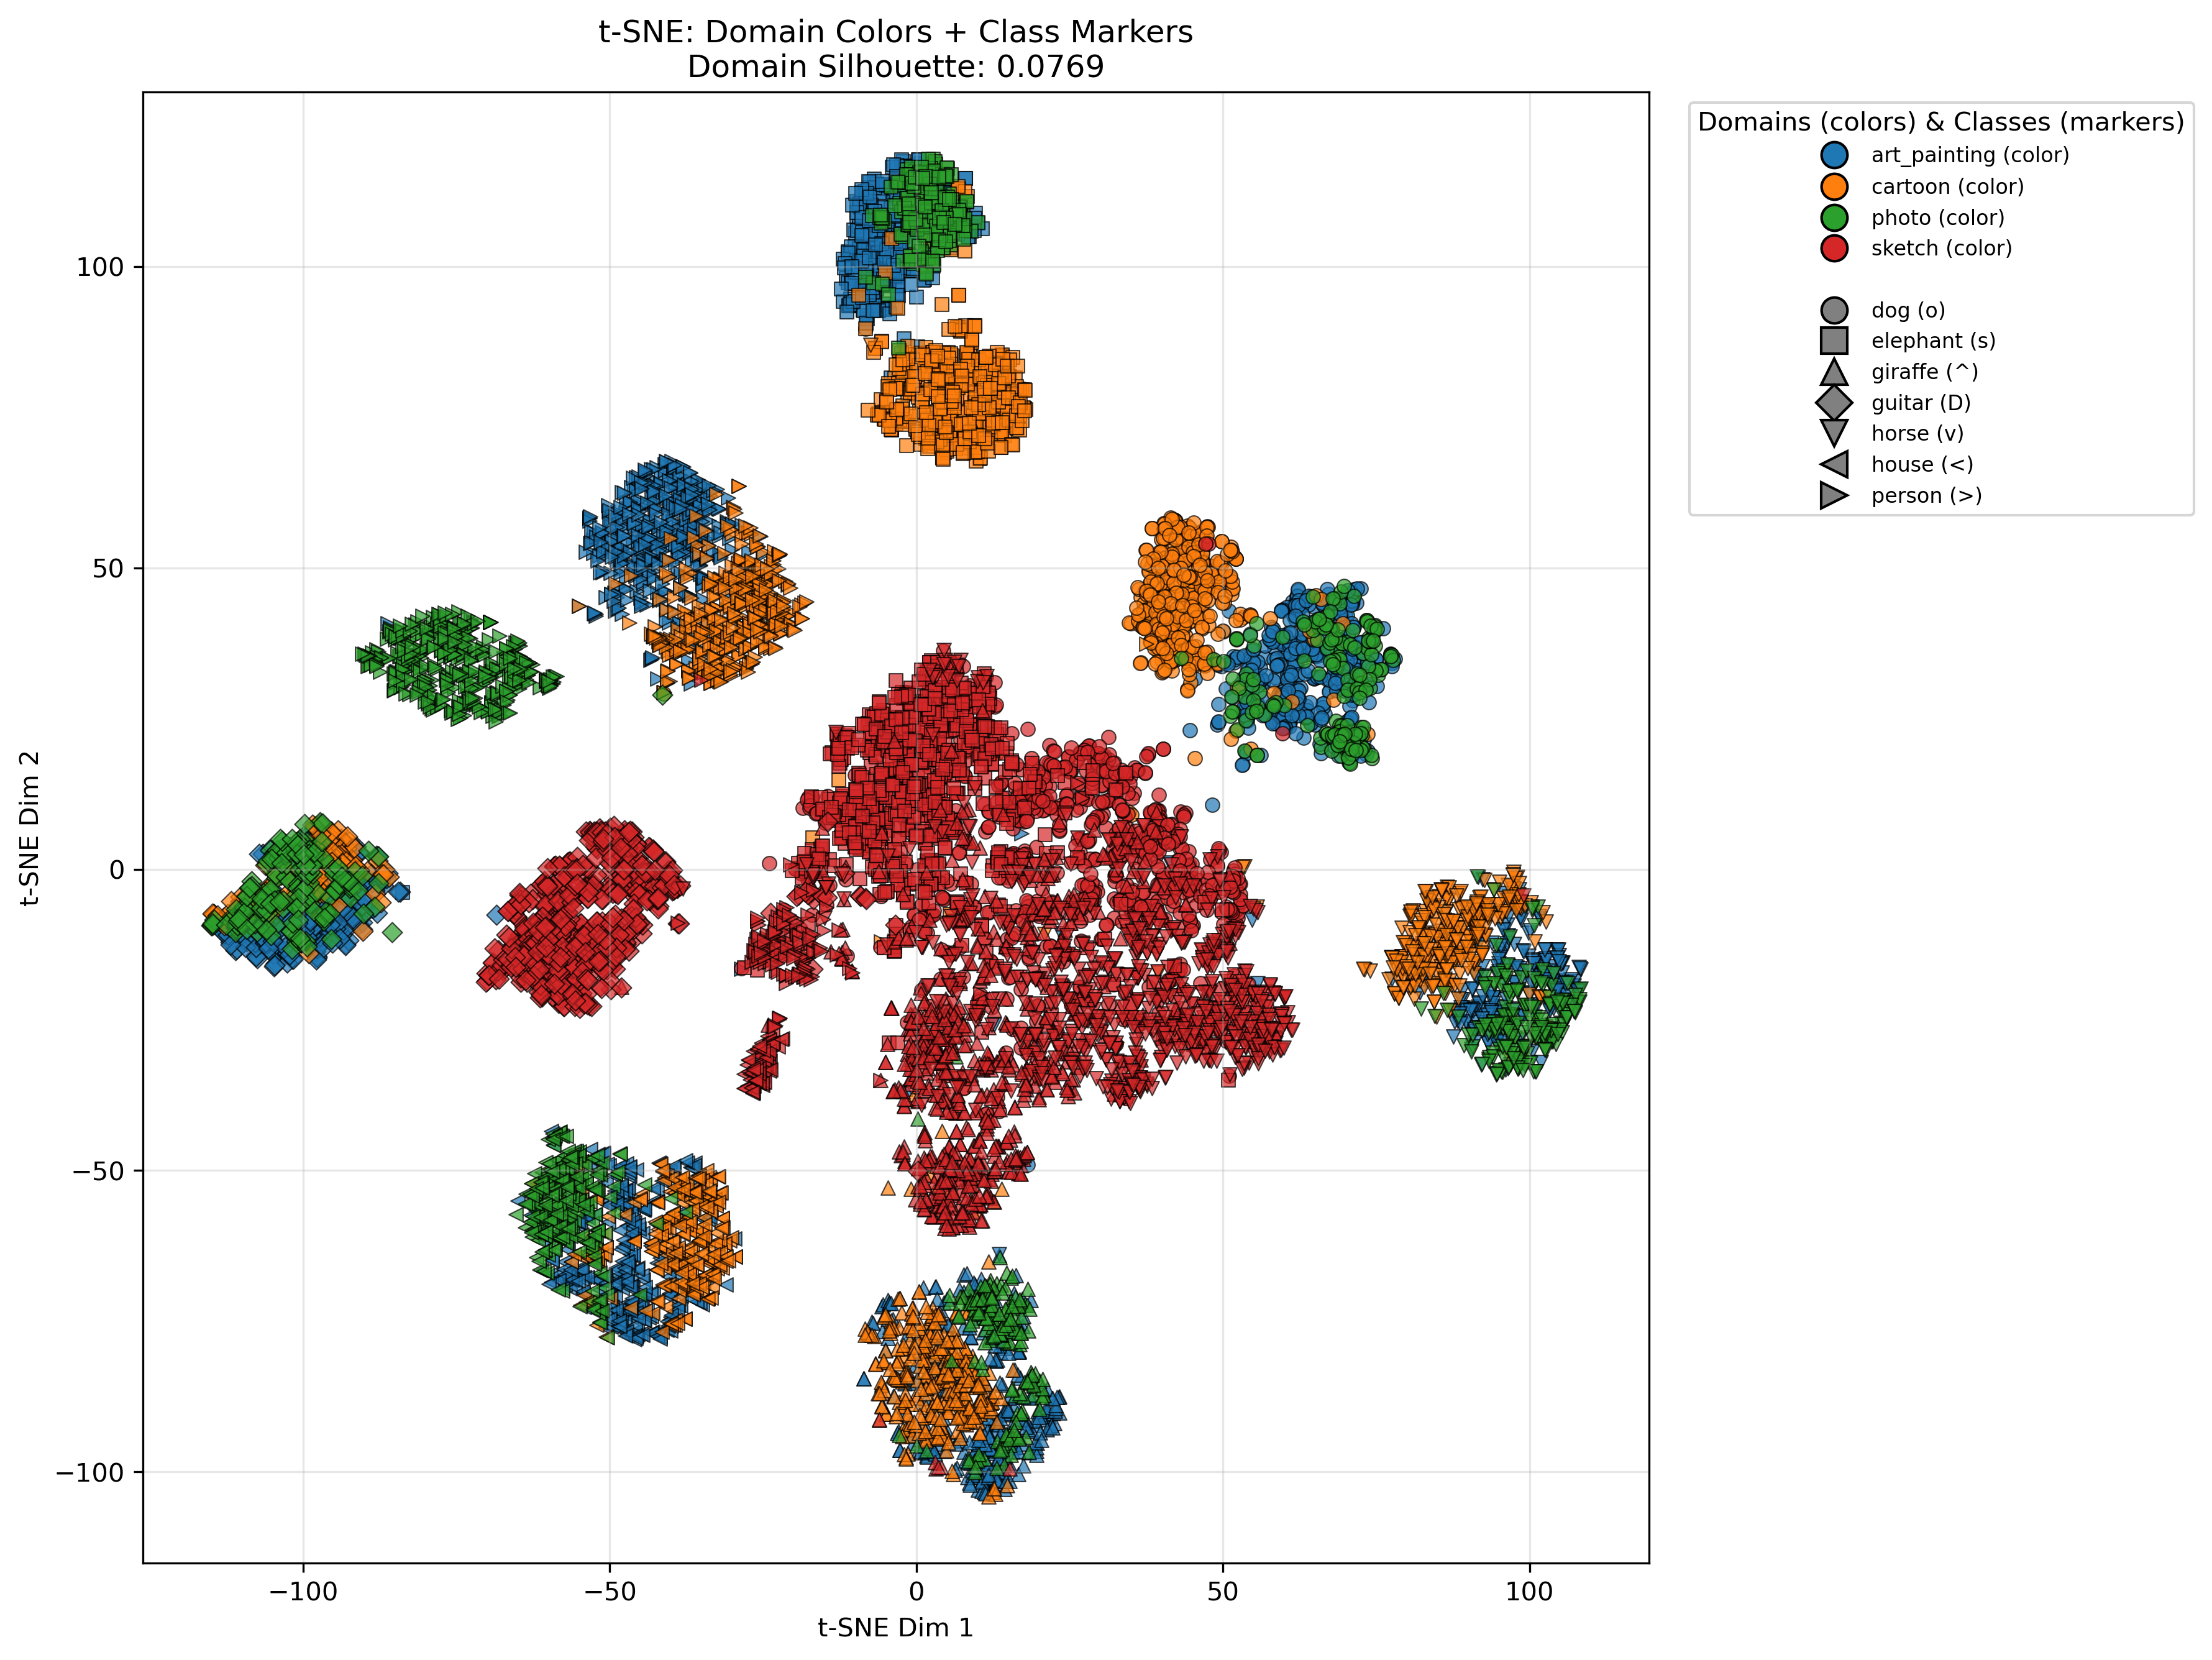
\includegraphics[width=.95\textwidth]{images/tsne_pacs_resnet50_fc512_ms12_a0d1_.png}
    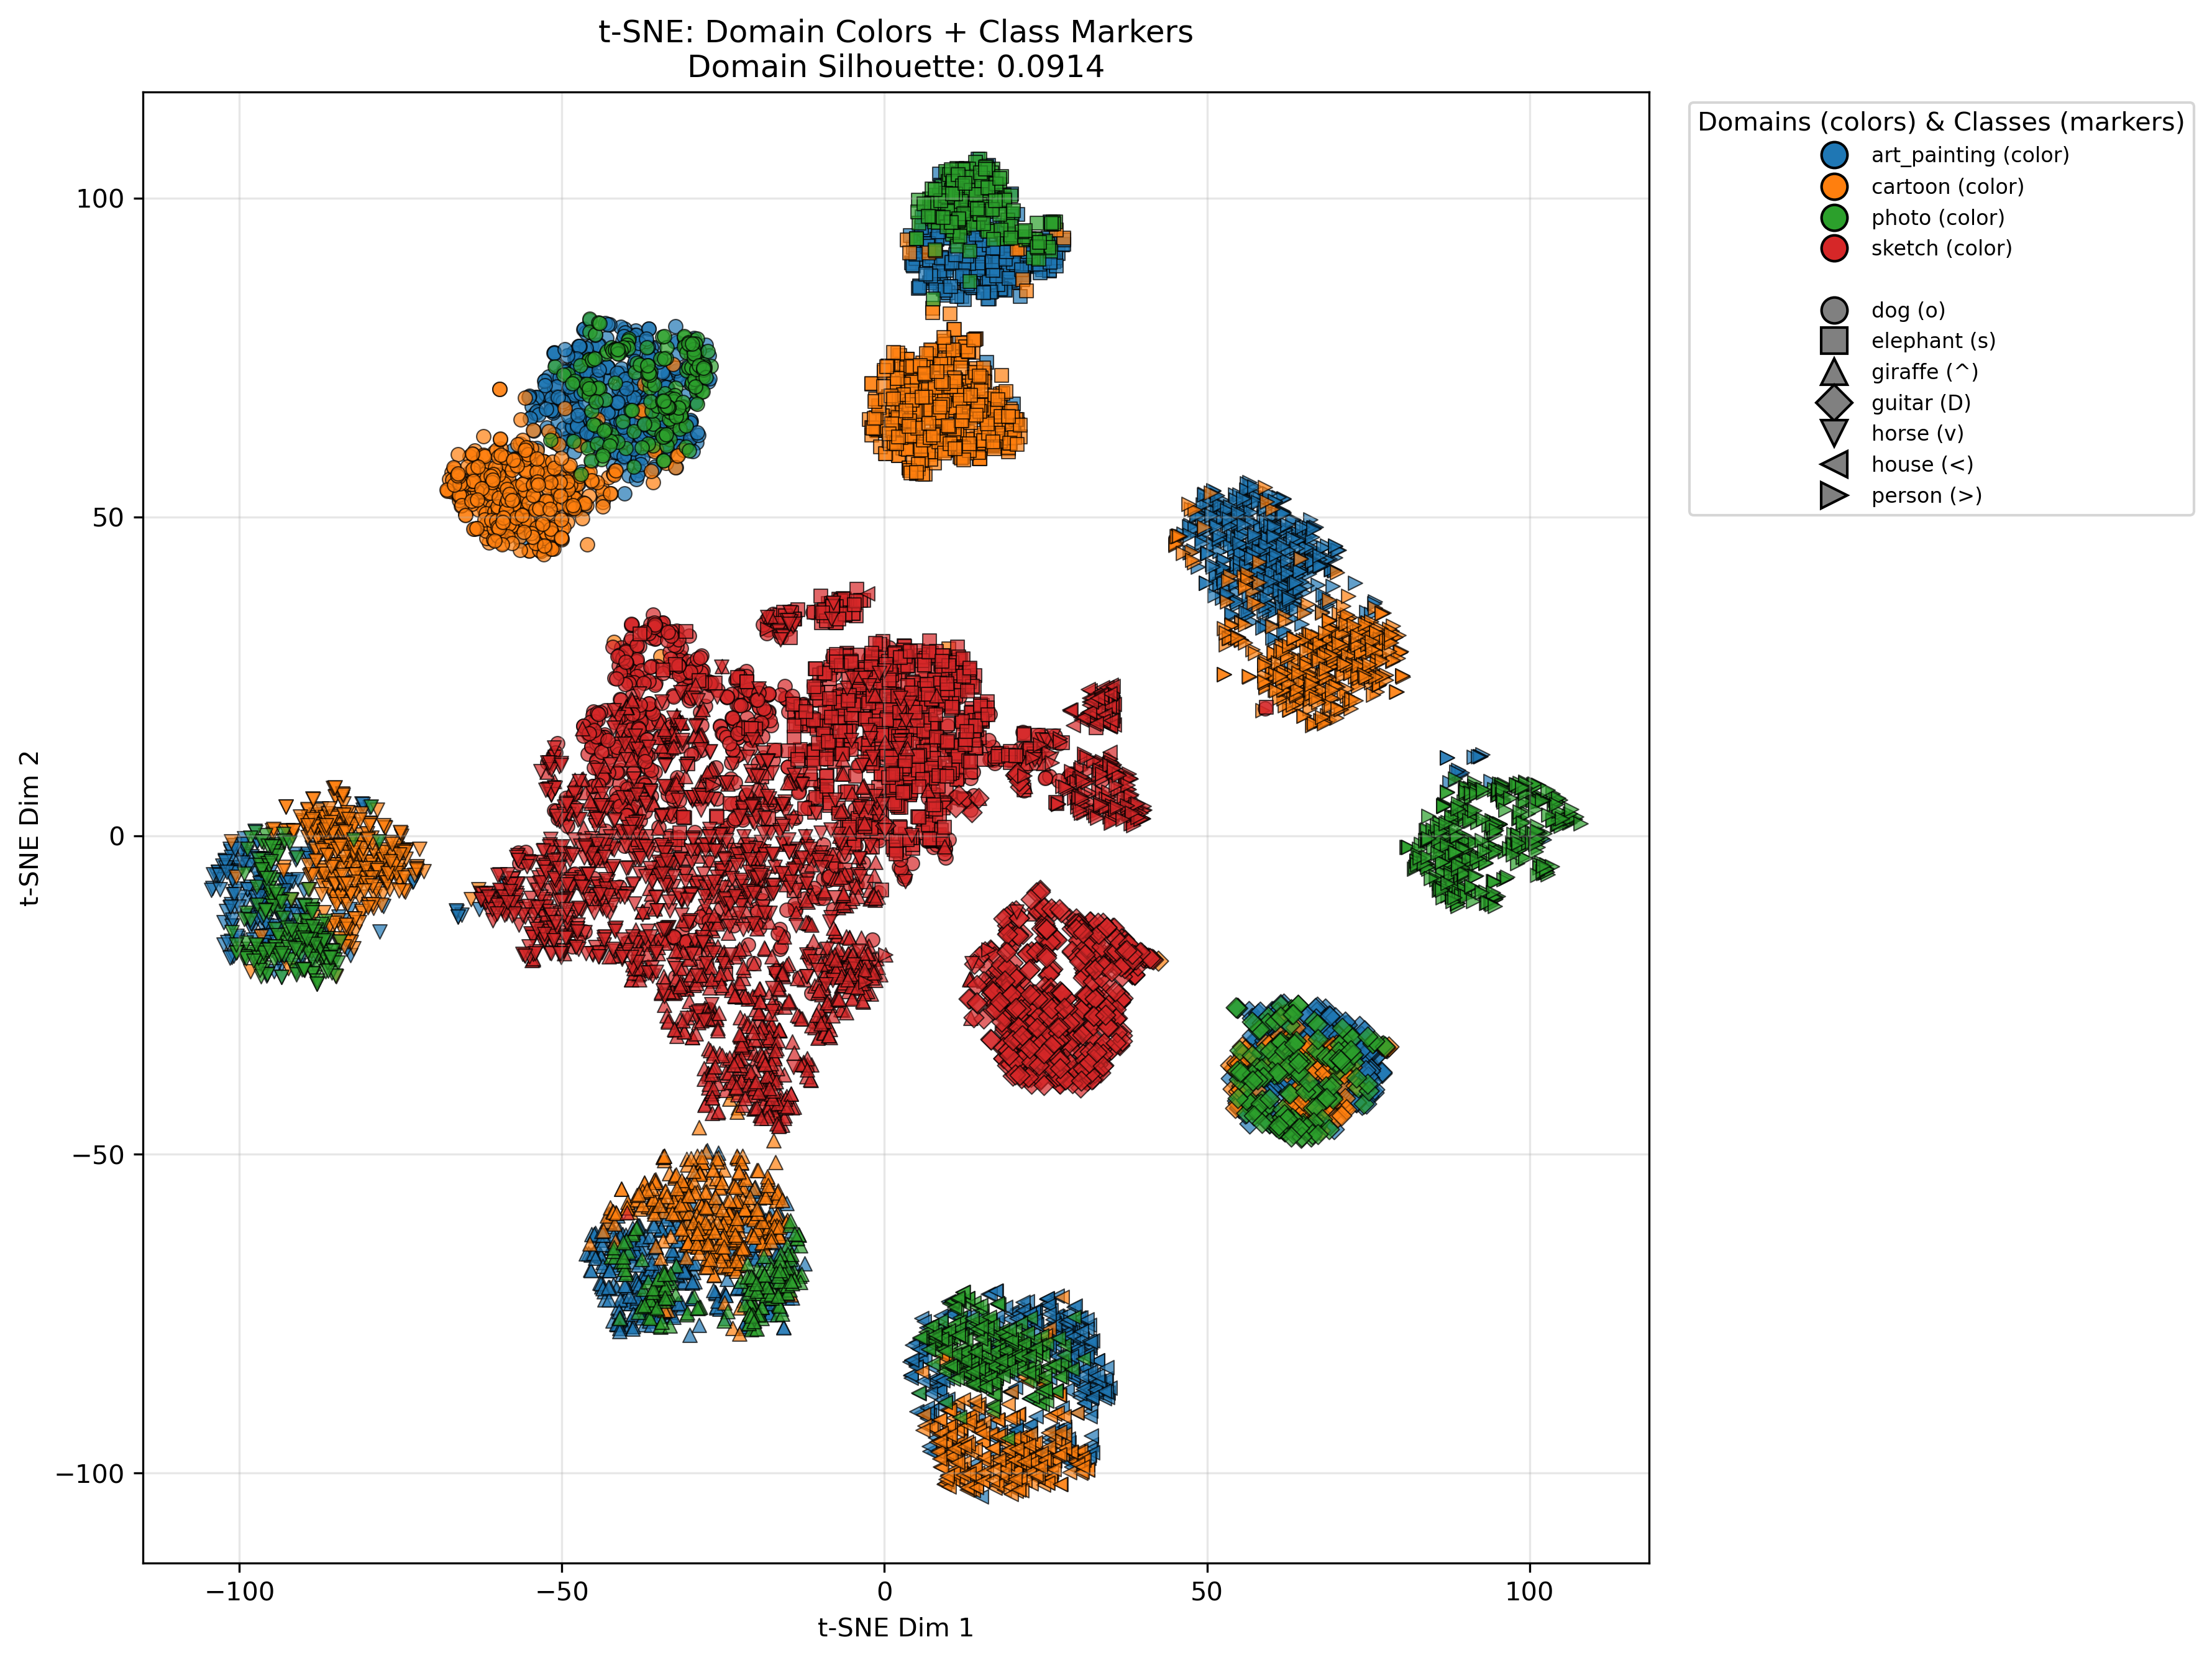
\includegraphics[width=.95\textwidth]{images/tsne_pacs_resnet50_fc512_.png}
    \caption{tSNE evaluation from the output of an introduced 512-dimensional fully connected layer right before the classification layer of a ResNet-50 model with (top) and without (bottom) Mixstyle after the first two layers, respectively. For both models, sketch (red) was used as validation domain.}
    \label{fig:tSNE}
\end{figure}

\subsection{Ablation Studies}

\begin{table}[t]
    \centering
    \begin{minipage}[t]{0.48\textwidth}
        \centering
        \caption{Results of an ablation study on a threefold split of PACS into train, validation and test set. Results are given as mean $\pm$ standard deviation of percent accuracy. The model used was ResNet-50 + FC + MS1\&2 + FR1.}
        \label{tab:results_threefold}
        \vspace{.5em}
        \begin{tabular}{l c}
            \toprule
            Art painting & $73.08 \pm 4.52$ \\
            Cartoon & $74.69 \pm 0.26$ \\
            Photo & $97.32 \pm 0.15$ \\
            Sketch & $70.54 \pm 2.95$ \\
            \midrule
            Total & $78.90 \pm 1.70$ \\
            \bottomrule
        \end{tabular}
    \end{minipage}
    \hfill
    \begin{minipage}[t]{0.48\textwidth}
        \centering
        \caption{Results of one run on Office-Home with the model ResNet-50 + FC + MS1\&2. Due to computational and time constraints, only one run was evaluated. Results are given as percent accuracy.}
        \label{tab:results_office-home}
        \vspace{.5em}
        \begin{tabular}{l c}
            \toprule
            Art & $63.29$ \\
            Clip art & $48.74$ \\
            Product & $73.89$ \\
            Real World & $76.29$ \\
            \midrule
            Total & $65.55$ \\
            \bottomrule
        \end{tabular}
    \end{minipage}
\end{table}

In a first ablation study, we split the dataset into three parts. One domain was used for validation, one for testing and two for training. We iterated through the domains to select a test domain. The validation domain was chosen among the remaining domains at random. The results are shown in table \ref{tab:results_threefold}. This experiment is again a great illustration that the photo domain brings no insight because of the use of pretrained weights. It is however interesting to see that the other three domains have much more similar performance than in the twofold split.

We additionally evaluated one model on the Office-Home dataset. Due to time constraints, we were only able to run one seed as that takes about 7 hours on our hardware to complete. Table \ref{tab:results_office-home} lists the results. Office-Home has 65 classes, so a worse performance than on PACS was to be expected. Overall, however, the accuracy here is quite high and again confirms the results of \cite{mixstyle_ref}.
